\begin{comment}
\documentclass[10pt]{article}
\usepackage{fullpage, graphicx, url}
\setlength{\parskip}{1ex}
\setlength{\parindent}{0ex}
\title{FLcount}
\begin{document}


\begin{tabular}{ccc}
The Alternative Csound Reference Manual & & \\
Previous & &Next

\end{tabular}

%\hline 
\end{comment}
\section{FLcount}
FLcount�--� A FLTK widget opcode that creates a counter. \subsection*{Description}


  Allows the user to increase/decrease a value with mouse clicks on a corresponding arrow button. 
\subsection*{Syntax}


 kout, ihandle \textbf{FLcount}
 ``label'', imin, imax, istep1, istep2, itype, iwidth, iheight, ix, iy, iopcode [, kp1] [, kp2] [, kp3] [...] [, kpN]
\subsection*{Initialization}


 \emph{ihandle}
 -- a handle value (an integer number) that unequivocally references a corresponding widget. Used by further opcodes that changes some valuator's properties. It is automatically set by the corresponding valuator. 


 \emph{``label''}
 -- a double-quoted string containing some user-provided text, placed near the corresponding widget. 


 \emph{imin}
 -- minimum value of output range 


 \emph{imax}
 -- maximum value of output range 


 \emph{istep1}
 -- a floating-point number indicating the increment of valuator value corresponding to of each mouse click. \emph{istep1}
 is for coarse adjustments. 


 \emph{istep2}
 -- a floating-point number indicating the increment of valuator value corresponding to of each mouse click. \emph{istep2}
 is for fine adjustments. 


 \emph{itype}
 -- an integer number denoting the appearance of the valuator. 


 \emph{iwidth}
 -- width of widget. 


 \emph{iheight}
 -- height of widget. 


 \emph{ix}
 -- horizontal position of upper left corner of the valuator, relative to the upper left corner of corresponding window (expressed in pixels). 


 \emph{iy}
 -- vertical position of upper left corner of the valuator, relative to the upper left corner of corresponding window (expressed in pixels). 


 \emph{iopcode}
 -- score opcode type. You have to provide the ascii code of the letter corresponding to the score opcode. At present time only ``i'' (ascii code 105) score statements are supported. A zero value refers to a default value of ``i''. So both 0 and 105 activates the \emph{i}
 opcode. A value of -1 disables this opcode feature. 
\subsection*{Performance}


 \emph{kout}
 -- output value 


 \emph{kp1}
, \emph{kp2}
, ..., \emph{kpN}
 -- arguments of the activated instruments. 


 \emph{FLcount}
 allows the user to increase/decrease a value with mouse clicks on corresponding arrow buttons: 


 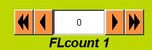
\includegraphics[scale=1]{flcount} 


 FLcount.


  There are two kind of arrow buttons, for larger and smaller steps. Notice that \emph{FLcount}
 not only outputs a value and a handle, but can also activate (schedule) an instrument provided by the user each time a button is pressed. P-fields of the activated instrument are \emph{kp1}
 (instrument number), \emph{kp2}
 (action time), \emph{kp3}
 (duration) and so on with user p-fields. If the \emph{iopcode}
 argument is set to a negative number, no instrument is activated. So this feature is optional. 
\subsection*{Examples}


  Here is an example of the flcount opcode. It uses the files \emph{flcount.orc}
 and \emph{flcount.sco}
. 


 \textbf{Example 1. Example of the flcount opcode.}

\begin{lstlisting}
/* flcount.orc */
; Demonstration of the flcount opcode
; clicking on the single arrow buttons
; increments the oscillator in semitone steps
; clicking on the double arrow buttons 
; increments the oscillator in octave steps
sr = 44100
kr = 441
ksmps = 100
nchnls = 1

FLpanel "Counter", 900, 400, 50, 50
    ; Minimum value output by counter
    imin = 6
    ; Maximum value output by counter
    imax = 12
    ; Single arrow step size (semitones)
    istep1 = 1/12
    ; Double arrow step size (octave)
    istep2 = 1 
    ; Counter type (1=double arrow counter)
    itype = 1
    ; Width of the counter in pixels
    iwidth = 200
    ; Height of the counter in pixels
    iheight = 30
    ; Distance of the left edge of the counter
    ; from the left edge of the panel
    ix = 50
    ; Distance of the top edge of the counter
    ; from the top edge of the panel
    iy = 50
    ; Score event type (-1=ignored)
    iopcode = -1

    gkoct, ihandle FLcount "pitch in oct format", imin, imax, istep1, istep2, itype, iwidth, iheight, ix, iy, iopcode, 1, 0, 1
; End of panel contents
FLpanelEnd
; Run the widget thread!
FLrun

instr 1
    iamp = 15000
    ifn = 1
    asig oscili iamp, cpsoct(gkoct), ifn
    out asig
endin
/* flcount.orc */
        
\end{lstlisting}
\begin{lstlisting}
/* flcount.sco */
; Function table that defines a single cycle
; of a sine wave.
f 1 0 1024 10 1

; Instrument 1 will play a note for 1 hour.
i 1 0 3600
e
/* flcount.sco */
        
\end{lstlisting}
\subsection*{See Also}


 \emph{FLjoy}
, \emph{FLkeyb}
, \emph{FLknob}
, \emph{FLroller}
, \emph{FLslider}
, \emph{FLtext}

\subsection*{Credits}


 Author: Gabriel Maldonado


 New in version 4.22


 Example written by Iain McCurdy, edited by Kevin Conder.
%\hline 


\begin{comment}
\begin{tabular}{lcr}
Previous &Home &Next \\
FLcolor2 &Up &FLgetsnap

\end{tabular}


\end{document}
\end{comment}
